% Created by tikzDevice version 0.12.3 on 2020-05-30 12:36:49
% !TEX encoding = UTF-8 Unicode
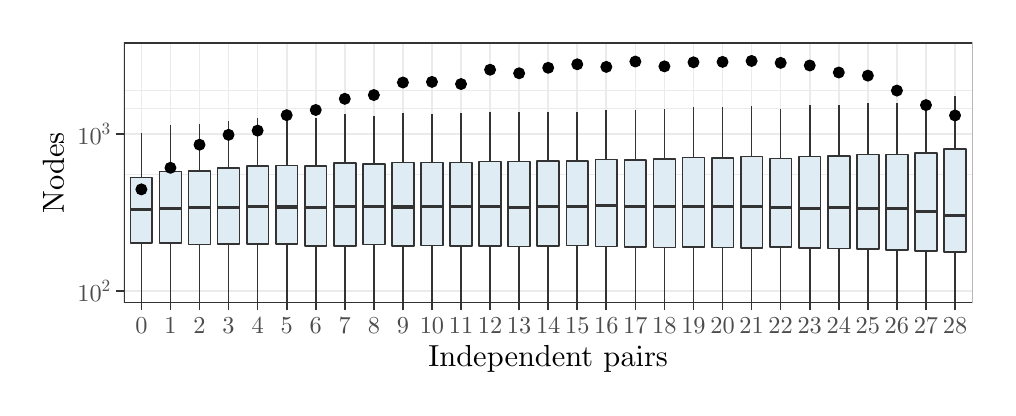
\begin{tikzpicture}[x=1pt,y=1pt]
\definecolor{fillColor}{RGB}{255,255,255}
\path[use as bounding box,fill=fillColor,fill opacity=0.00] (0,0) rectangle (346.90,130.09);
\begin{scope}
\path[clip] (  0.00,  0.00) rectangle (346.90,130.09);
\definecolor{drawColor}{RGB}{255,255,255}
\definecolor{fillColor}{RGB}{255,255,255}

\path[draw=drawColor,line width= 0.6pt,line join=round,line cap=round,fill=fillColor] (  0.00,  0.00) rectangle (346.90,130.09);
\end{scope}
\begin{scope}
\path[clip] ( 34.79, 30.69) rectangle (341.40,124.59);
\definecolor{fillColor}{RGB}{255,255,255}

\path[fill=fillColor] ( 34.79, 30.69) rectangle (341.40,124.59);
\definecolor{drawColor}{gray}{0.92}

\path[draw=drawColor,line width= 0.3pt,line join=round] ( 34.79, 77.01) --
	(341.40, 77.01);

\path[draw=drawColor,line width= 0.3pt,line join=round] ( 34.79,100.92) --
	(341.40,100.92);

\path[draw=drawColor,line width= 0.3pt,line join=round] ( 34.79,107.58) --
	(341.40,107.58);

\path[draw=drawColor,line width= 0.6pt,line join=round] ( 34.79, 34.95) --
	(341.40, 34.95);

\path[draw=drawColor,line width= 0.6pt,line join=round] ( 34.79, 91.75) --
	(341.40, 91.75);

\path[draw=drawColor,line width= 0.6pt,line join=round] ( 41.09, 30.69) --
	( 41.09,124.59);

\path[draw=drawColor,line width= 0.6pt,line join=round] ( 51.59, 30.69) --
	( 51.59,124.59);

\path[draw=drawColor,line width= 0.6pt,line join=round] ( 62.09, 30.69) --
	( 62.09,124.59);

\path[draw=drawColor,line width= 0.6pt,line join=round] ( 72.59, 30.69) --
	( 72.59,124.59);

\path[draw=drawColor,line width= 0.6pt,line join=round] ( 83.09, 30.69) --
	( 83.09,124.59);

\path[draw=drawColor,line width= 0.6pt,line join=round] ( 93.59, 30.69) --
	( 93.59,124.59);

\path[draw=drawColor,line width= 0.6pt,line join=round] (104.09, 30.69) --
	(104.09,124.59);

\path[draw=drawColor,line width= 0.6pt,line join=round] (114.59, 30.69) --
	(114.59,124.59);

\path[draw=drawColor,line width= 0.6pt,line join=round] (125.09, 30.69) --
	(125.09,124.59);

\path[draw=drawColor,line width= 0.6pt,line join=round] (135.59, 30.69) --
	(135.59,124.59);

\path[draw=drawColor,line width= 0.6pt,line join=round] (146.09, 30.69) --
	(146.09,124.59);

\path[draw=drawColor,line width= 0.6pt,line join=round] (156.59, 30.69) --
	(156.59,124.59);

\path[draw=drawColor,line width= 0.6pt,line join=round] (167.09, 30.69) --
	(167.09,124.59);

\path[draw=drawColor,line width= 0.6pt,line join=round] (177.59, 30.69) --
	(177.59,124.59);

\path[draw=drawColor,line width= 0.6pt,line join=round] (188.09, 30.69) --
	(188.09,124.59);

\path[draw=drawColor,line width= 0.6pt,line join=round] (198.59, 30.69) --
	(198.59,124.59);

\path[draw=drawColor,line width= 0.6pt,line join=round] (209.09, 30.69) --
	(209.09,124.59);

\path[draw=drawColor,line width= 0.6pt,line join=round] (219.59, 30.69) --
	(219.59,124.59);

\path[draw=drawColor,line width= 0.6pt,line join=round] (230.09, 30.69) --
	(230.09,124.59);

\path[draw=drawColor,line width= 0.6pt,line join=round] (240.59, 30.69) --
	(240.59,124.59);

\path[draw=drawColor,line width= 0.6pt,line join=round] (251.09, 30.69) --
	(251.09,124.59);

\path[draw=drawColor,line width= 0.6pt,line join=round] (261.59, 30.69) --
	(261.59,124.59);

\path[draw=drawColor,line width= 0.6pt,line join=round] (272.09, 30.69) --
	(272.09,124.59);

\path[draw=drawColor,line width= 0.6pt,line join=round] (282.60, 30.69) --
	(282.60,124.59);

\path[draw=drawColor,line width= 0.6pt,line join=round] (293.10, 30.69) --
	(293.10,124.59);

\path[draw=drawColor,line width= 0.6pt,line join=round] (303.60, 30.69) --
	(303.60,124.59);

\path[draw=drawColor,line width= 0.6pt,line join=round] (314.10, 30.69) --
	(314.10,124.59);

\path[draw=drawColor,line width= 0.6pt,line join=round] (324.60, 30.69) --
	(324.60,124.59);

\path[draw=drawColor,line width= 0.6pt,line join=round] (335.10, 30.69) --
	(335.10,124.59);
\definecolor{drawColor}{gray}{0.20}

\path[draw=drawColor,line width= 0.6pt,line join=round] ( 41.09, 75.95) --
	( 41.09, 92.07);

\path[draw=drawColor,line width= 0.6pt,line join=round] ( 41.09, 52.30) --
	( 41.09, 43.78) --
	( 41.09, 30.65) --
	( 41.09,  0.76);
\definecolor{fillColor}{RGB}{224,236,244}

\path[draw=drawColor,line width= 0.6pt,line join=round,line cap=round,fill=fillColor] ( 37.15, 75.95) --
	( 37.15, 52.30) --
	( 41.09, 52.30) --
	( 45.03, 52.30) --
	( 45.03, 75.95) --
	( 41.09, 75.95) --
	( 37.15, 75.95) --
	cycle;

\path[draw=drawColor,line width= 1.1pt,line join=round] ( 37.15, 64.33) --
	( 41.09, 64.33) --
	( 45.03, 64.33);

\path[draw=drawColor,line width= 0.6pt,line join=round] ( 51.59, 78.10) --
	( 51.59, 94.85);

\path[draw=drawColor,line width= 0.6pt,line join=round] ( 51.59, 52.30) --
	( 51.59, 39.14) --
	( 51.59,  9.06);

\path[draw=drawColor,line width= 0.6pt,line join=round,line cap=round,fill=fillColor] ( 47.65, 78.10) --
	( 47.65, 52.30) --
	( 51.59, 52.30) --
	( 55.53, 52.30) --
	( 55.53, 78.10) --
	( 51.59, 78.10) --
	( 47.65, 78.10) --
	cycle;

\path[draw=drawColor,line width= 1.1pt,line join=round] ( 47.65, 64.78) --
	( 51.59, 64.78) --
	( 55.53, 64.78);

\path[draw=drawColor,line width= 0.6pt,line join=round] ( 62.09, 78.40) --
	( 62.09, 95.33);

\path[draw=drawColor,line width= 0.6pt,line join=round] ( 62.09, 51.68) --
	( 62.09, 37.75) --
	( 62.09,  2.66);

\path[draw=drawColor,line width= 0.6pt,line join=round,line cap=round,fill=fillColor] ( 58.15, 78.40) --
	( 58.15, 51.68) --
	( 62.09, 51.68) --
	( 66.03, 51.68) --
	( 66.03, 78.40) --
	( 62.09, 78.40) --
	( 58.15, 78.40) --
	cycle;

\path[draw=drawColor,line width= 1.1pt,line join=round] ( 58.15, 65.00) --
	( 62.09, 65.00) --
	( 66.03, 65.00);

\path[draw=drawColor,line width= 0.6pt,line join=round] ( 72.59, 79.27) --
	( 72.59, 96.45);

\path[draw=drawColor,line width= 0.6pt,line join=round] ( 72.59, 51.80) --
	( 72.59, 38.19) --
	( 72.59,  5.26);

\path[draw=drawColor,line width= 0.6pt,line join=round,line cap=round,fill=fillColor] ( 68.65, 79.27) --
	( 68.65, 51.80) --
	( 72.59, 51.80) --
	( 76.53, 51.80) --
	( 76.53, 79.27) --
	( 72.59, 79.27) --
	( 68.65, 79.27) --
	cycle;

\path[draw=drawColor,line width= 1.1pt,line join=round] ( 68.65, 65.00) --
	( 72.59, 65.00) --
	( 76.53, 65.00);

\path[draw=drawColor,line width= 0.6pt,line join=round] ( 83.09, 80.00) --
	( 83.09, 97.36);

\path[draw=drawColor,line width= 0.6pt,line join=round] ( 83.09, 51.80) --
	( 83.09, 38.19) --
	( 83.09,  5.26);

\path[draw=drawColor,line width= 0.6pt,line join=round,line cap=round,fill=fillColor] ( 79.15, 80.00) --
	( 79.15, 51.80) --
	( 83.09, 51.80) --
	( 87.03, 51.80) --
	( 87.03, 80.00) --
	( 83.09, 80.00) --
	( 79.15, 80.00) --
	cycle;

\path[draw=drawColor,line width= 1.1pt,line join=round] ( 79.15, 65.50) --
	( 83.09, 65.50) --
	( 87.03, 65.50);

\path[draw=drawColor,line width= 0.6pt,line join=round] ( 93.59, 80.28) --
	( 93.59, 97.67);

\path[draw=drawColor,line width= 0.6pt,line join=round] ( 93.59, 51.93) --
	( 93.59, 38.08) --
	( 93.59,  3.55);

\path[draw=drawColor,line width= 0.6pt,line join=round,line cap=round,fill=fillColor] ( 89.65, 80.28) --
	( 89.65, 51.93) --
	( 93.59, 51.93) --
	( 97.53, 51.93) --
	( 97.53, 80.28) --
	( 93.59, 80.28) --
	( 89.65, 80.28) --
	cycle;

\path[draw=drawColor,line width= 1.1pt,line join=round] ( 89.65, 65.29) --
	( 93.59, 65.29) --
	( 97.53, 65.29);

\path[draw=drawColor,line width= 0.6pt,line join=round] (104.09, 80.04) --
	(104.09, 97.53);

\path[draw=drawColor,line width= 0.6pt,line join=round] (104.09, 51.30) --
	(104.09, 37.75) --
	(104.09,  5.26);

\path[draw=drawColor,line width= 0.6pt,line join=round,line cap=round,fill=fillColor] (100.15, 80.04) --
	(100.15, 51.30) --
	(104.09, 51.30) --
	(108.03, 51.30) --
	(108.03, 80.04) --
	(104.09, 80.04) --
	(100.15, 80.04) --
	cycle;

\path[draw=drawColor,line width= 1.1pt,line join=round] (100.15, 65.00) --
	(104.09, 65.00) --
	(108.03, 65.00);

\path[draw=drawColor,line width= 0.6pt,line join=round] (114.59, 81.09) --
	(114.59, 98.81);

\path[draw=drawColor,line width= 0.6pt,line join=round] (114.59, 51.30) --
	(114.59, 37.97) --
	(114.59,  6.85);

\path[draw=drawColor,line width= 0.6pt,line join=round,line cap=round,fill=fillColor] (110.66, 81.09) --
	(110.66, 51.30) --
	(114.59, 51.30) --
	(118.53, 51.30) --
	(118.53, 81.09) --
	(114.59, 81.09) --
	(110.66, 81.09) --
	cycle;

\path[draw=drawColor,line width= 1.1pt,line join=round] (110.66, 65.36) --
	(114.59, 65.36) --
	(118.53, 65.36);

\path[draw=drawColor,line width= 0.6pt,line join=round] (125.09, 80.74) --
	(125.09, 98.30);

\path[draw=drawColor,line width= 0.6pt,line join=round] (125.09, 51.68) --
	(125.09, 38.62) --
	(125.09,  9.06);

\path[draw=drawColor,line width= 0.6pt,line join=round,line cap=round,fill=fillColor] (121.16, 80.74) --
	(121.16, 51.68) --
	(125.09, 51.68) --
	(129.03, 51.68) --
	(129.03, 80.74) --
	(125.09, 80.74) --
	(121.16, 80.74) --
	cycle;

\path[draw=drawColor,line width= 1.1pt,line join=round] (121.16, 65.43) --
	(125.09, 65.43) --
	(129.03, 65.43);

\path[draw=drawColor,line width= 0.6pt,line join=round] (135.59, 81.32) --
	(135.59, 99.08);

\path[draw=drawColor,line width= 0.6pt,line join=round] (135.59, 51.30) --
	(135.59, 37.64) --
	(135.59,  4.42);

\path[draw=drawColor,line width= 0.6pt,line join=round,line cap=round,fill=fillColor] (131.66, 81.32) --
	(131.66, 51.30) --
	(135.59, 51.30) --
	(139.53, 51.30) --
	(139.53, 81.32) --
	(135.59, 81.32) --
	(131.66, 81.32) --
	cycle;

\path[draw=drawColor,line width= 1.1pt,line join=round] (131.66, 65.29) --
	(135.59, 65.29) --
	(139.53, 65.29);

\path[draw=drawColor,line width= 0.6pt,line join=round] (146.09, 81.32) --
	(146.09, 98.97);

\path[draw=drawColor,line width= 0.6pt,line join=round] (146.09, 51.43) --
	(146.09, 42.90) --
	(146.09, 29.76) --
	(146.09,  0.00);

\path[draw=drawColor,line width= 0.6pt,line join=round,line cap=round,fill=fillColor] (142.16, 81.32) --
	(142.16, 51.43) --
	(146.09, 51.43) --
	(150.03, 51.43) --
	(150.03, 81.32) --
	(146.09, 81.32) --
	(142.16, 81.32) --
	cycle;

\path[draw=drawColor,line width= 1.1pt,line join=round] (142.16, 65.64) --
	(146.09, 65.64) --
	(150.03, 65.64);

\path[draw=drawColor,line width= 0.6pt,line join=round] (156.59, 81.39) --
	(156.59, 99.17);

\path[draw=drawColor,line width= 0.6pt,line join=round] (156.59, 51.30) --
	(156.59, 37.97) --
	(156.59,  6.85);

\path[draw=drawColor,line width= 0.6pt,line join=round,line cap=round,fill=fillColor] (152.66, 81.39) --
	(152.66, 51.30) --
	(156.59, 51.30) --
	(160.53, 51.30) --
	(160.53, 81.39) --
	(156.59, 81.39) --
	(152.66, 81.39) --
	cycle;

\path[draw=drawColor,line width= 1.1pt,line join=round] (152.66, 65.64) --
	(156.59, 65.64) --
	(160.53, 65.64);

\path[draw=drawColor,line width= 0.6pt,line join=round] (167.09, 81.77) --
	(167.09, 99.66);

\path[draw=drawColor,line width= 0.6pt,line join=round] (167.09, 51.17) --
	(167.09, 37.53) --
	(167.09,  4.42);

\path[draw=drawColor,line width= 0.6pt,line join=round,line cap=round,fill=fillColor] (163.16, 81.77) --
	(163.16, 51.17) --
	(167.09, 51.17) --
	(171.03, 51.17) --
	(171.03, 81.77) --
	(167.09, 81.77) --
	(163.16, 81.77) --
	cycle;

\path[draw=drawColor,line width= 1.1pt,line join=round] (163.16, 65.43) --
	(167.09, 65.43) --
	(171.03, 65.43);

\path[draw=drawColor,line width= 0.6pt,line join=round] (177.59, 81.73) --
	(177.59, 99.63);

\path[draw=drawColor,line width= 0.6pt,line join=round] (177.59, 51.05) --
	(177.59, 37.64) --
	(177.59,  6.06);

\path[draw=drawColor,line width= 0.6pt,line join=round,line cap=round,fill=fillColor] (173.66, 81.73) --
	(173.66, 51.05) --
	(177.59, 51.05) --
	(181.53, 51.05) --
	(181.53, 81.73) --
	(177.59, 81.73) --
	(173.66, 81.73) --
	cycle;

\path[draw=drawColor,line width= 1.1pt,line join=round] (173.66, 65.14) --
	(177.59, 65.14) --
	(181.53, 65.14);

\path[draw=drawColor,line width= 0.6pt,line join=round] (188.09, 81.95) --
	(188.09, 99.79);

\path[draw=drawColor,line width= 0.6pt,line join=round] (188.09, 51.17) --
	(188.09, 37.97) --
	(188.09,  7.61);

\path[draw=drawColor,line width= 0.6pt,line join=round,line cap=round,fill=fillColor] (184.16, 81.95) --
	(184.16, 51.17) --
	(188.09, 51.17) --
	(192.03, 51.17) --
	(192.03, 81.95) --
	(188.09, 81.95) --
	(184.16, 81.95) --
	cycle;

\path[draw=drawColor,line width= 1.1pt,line join=round] (184.16, 65.43) --
	(188.09, 65.43) --
	(192.03, 65.43);

\path[draw=drawColor,line width= 0.6pt,line join=round] (198.59, 81.87) --
	(198.59, 99.71);

\path[draw=drawColor,line width= 0.6pt,line join=round] (198.59, 51.43) --
	(198.59, 38.19) --
	(198.59,  7.61);

\path[draw=drawColor,line width= 0.6pt,line join=round,line cap=round,fill=fillColor] (194.66, 81.87) --
	(194.66, 51.43) --
	(198.59, 51.43) --
	(202.53, 51.43) --
	(202.53, 81.87) --
	(198.59, 81.87) --
	(194.66, 81.87) --
	cycle;

\path[draw=drawColor,line width= 1.1pt,line join=round] (194.66, 65.64) --
	(198.59, 65.64) --
	(202.53, 65.64);

\path[draw=drawColor,line width= 0.6pt,line join=round] (209.09, 82.43) --
	(209.09,100.49);

\path[draw=drawColor,line width= 0.6pt,line join=round] (209.09, 51.05) --
	(209.09, 37.53) --
	(209.09,  5.26);

\path[draw=drawColor,line width= 0.6pt,line join=round,line cap=round,fill=fillColor] (205.16, 82.43) --
	(205.16, 51.05) --
	(209.09, 51.05) --
	(213.03, 51.05) --
	(213.03, 82.43) --
	(209.09, 82.43) --
	(205.16, 82.43) --
	cycle;

\path[draw=drawColor,line width= 1.1pt,line join=round] (205.16, 65.68) --
	(209.09, 65.68) --
	(213.03, 65.68);

\path[draw=drawColor,line width= 0.6pt,line join=round] (219.59, 82.36) --
	(219.59,100.38);

\path[draw=drawColor,line width= 0.6pt,line join=round] (219.59, 50.92) --
	(219.59, 37.97) --
	(219.59,  9.06);

\path[draw=drawColor,line width= 0.6pt,line join=round,line cap=round,fill=fillColor] (215.66, 82.36) --
	(215.66, 50.92) --
	(219.59, 50.92) --
	(223.53, 50.92) --
	(223.53, 82.36) --
	(219.59, 82.36) --
	(215.66, 82.36) --
	cycle;

\path[draw=drawColor,line width= 1.1pt,line join=round] (215.66, 65.43) --
	(219.59, 65.43) --
	(223.53, 65.43);

\path[draw=drawColor,line width= 0.6pt,line join=round] (230.09, 82.57) --
	(230.09,100.73);

\path[draw=drawColor,line width= 0.6pt,line join=round] (230.09, 50.66) --
	(230.09, 37.31) --
	(230.09,  6.06);

\path[draw=drawColor,line width= 0.6pt,line join=round,line cap=round,fill=fillColor] (226.16, 82.57) --
	(226.16, 50.66) --
	(230.09, 50.66) --
	(234.03, 50.66) --
	(234.03, 82.57) --
	(230.09, 82.57) --
	(226.16, 82.57) --
	cycle;

\path[draw=drawColor,line width= 1.1pt,line join=round] (226.16, 65.36) --
	(230.09, 65.36) --
	(234.03, 65.36);

\path[draw=drawColor,line width= 0.6pt,line join=round] (240.59, 83.13) --
	(240.59,101.31);

\path[draw=drawColor,line width= 0.6pt,line join=round] (240.59, 50.92) --
	(240.59, 37.53) --
	(240.59,  6.06);

\path[draw=drawColor,line width= 0.6pt,line join=round,line cap=round,fill=fillColor] (236.66, 83.13) --
	(236.66, 50.92) --
	(240.59, 50.92) --
	(244.53, 50.92) --
	(244.53, 83.13) --
	(240.59, 83.13) --
	(236.66, 83.13) --
	cycle;

\path[draw=drawColor,line width= 1.1pt,line join=round] (236.66, 65.50) --
	(240.59, 65.50) --
	(244.53, 65.50);

\path[draw=drawColor,line width= 0.6pt,line join=round] (251.09, 83.03) --
	(251.09,101.26);

\path[draw=drawColor,line width= 0.6pt,line join=round] (251.09, 50.66) --
	(251.09, 36.97) --
	(251.09,  3.55);

\path[draw=drawColor,line width= 0.6pt,line join=round,line cap=round,fill=fillColor] (247.16, 83.03) --
	(247.16, 50.66) --
	(251.09, 50.66) --
	(255.03, 50.66) --
	(255.03, 83.03) --
	(251.09, 83.03) --
	(247.16, 83.03) --
	cycle;

\path[draw=drawColor,line width= 1.1pt,line join=round] (247.16, 65.36) --
	(251.09, 65.36) --
	(255.03, 65.36);

\path[draw=drawColor,line width= 0.6pt,line join=round] (261.59, 83.55) --
	(261.59,101.89);

\path[draw=drawColor,line width= 0.6pt,line join=round] (261.59, 50.53) --
	(261.59, 36.97) --
	(261.59,  4.42);

\path[draw=drawColor,line width= 0.6pt,line join=round,line cap=round,fill=fillColor] (257.66, 83.55) --
	(257.66, 50.53) --
	(261.59, 50.53) --
	(265.53, 50.53) --
	(265.53, 83.55) --
	(261.59, 83.55) --
	(257.66, 83.55) --
	cycle;

\path[draw=drawColor,line width= 1.1pt,line join=round] (257.66, 65.36) --
	(261.59, 65.36) --
	(265.53, 65.36);

\path[draw=drawColor,line width= 0.6pt,line join=round] (272.09, 82.85) --
	(272.09,100.68);

\path[draw=drawColor,line width= 0.6pt,line join=round] (272.09, 50.79) --
	(272.09, 37.53) --
	(272.09,  6.85);

\path[draw=drawColor,line width= 0.6pt,line join=round,line cap=round,fill=fillColor] (268.16, 82.85) --
	(268.16, 50.79) --
	(272.09, 50.79) --
	(276.03, 50.79) --
	(276.03, 82.85) --
	(272.09, 82.85) --
	(268.16, 82.85) --
	cycle;

\path[draw=drawColor,line width= 1.1pt,line join=round] (268.16, 65.21) --
	(272.09, 65.21) --
	(276.03, 65.21);

\path[draw=drawColor,line width= 0.6pt,line join=round] (282.60, 83.58) --
	(282.60,101.97);

\path[draw=drawColor,line width= 0.6pt,line join=round] (282.60, 50.39) --
	(282.60, 37.08) --
	(282.60,  6.06);

\path[draw=drawColor,line width= 0.6pt,line join=round,line cap=round,fill=fillColor] (278.66, 83.58) --
	(278.66, 50.39) --
	(282.60, 50.39) --
	(286.53, 50.39) --
	(286.53, 83.58) --
	(282.60, 83.58) --
	(278.66, 83.58) --
	cycle;

\path[draw=drawColor,line width= 1.1pt,line join=round] (278.66, 64.78) --
	(282.60, 64.78) --
	(286.53, 64.78);

\path[draw=drawColor,line width= 0.6pt,line join=round] (293.10, 83.79) --
	(293.10,102.13);

\path[draw=drawColor,line width= 0.6pt,line join=round] (293.10, 50.26) --
	(293.10, 36.97) --
	(293.10,  6.06);

\path[draw=drawColor,line width= 0.6pt,line join=round,line cap=round,fill=fillColor] (289.16, 83.79) --
	(289.16, 72.33) --
	(289.16, 50.26) --
	(293.10, 50.26) --
	(297.03, 50.26) --
	(297.03, 72.33) --
	(297.03, 83.79) --
	(293.10, 83.79) --
	(289.16, 83.79) --
	cycle;

\path[draw=drawColor,line width= 1.1pt,line join=round] (289.16, 65.07) --
	(293.10, 65.07) --
	(297.03, 65.07);

\path[draw=drawColor,line width= 0.6pt,line join=round] (303.60, 84.22) --
	(303.60,102.80);

\path[draw=drawColor,line width= 0.6pt,line join=round] (303.60, 50.00) --
	(303.60, 37.31) --
	(303.60,  9.75);

\path[draw=drawColor,line width= 0.6pt,line join=round,line cap=round,fill=fillColor] (299.66, 84.22) --
	(299.66, 72.62) --
	(299.66, 50.00) --
	(303.60, 50.00) --
	(307.53, 50.00) --
	(307.53, 72.62) --
	(307.53, 84.22) --
	(303.60, 84.22) --
	(299.66, 84.22) --
	cycle;

\path[draw=drawColor,line width= 1.1pt,line join=round] (299.66, 64.78) --
	(303.60, 64.78) --
	(307.53, 64.78);

\path[draw=drawColor,line width= 0.6pt,line join=round] (314.10, 84.32) --
	(314.10,102.96);

\path[draw=drawColor,line width= 0.6pt,line join=round] (314.10, 49.73) --
	(314.10, 36.27) --
	(314.10,  4.42);

\path[draw=drawColor,line width= 0.6pt,line join=round,line cap=round,fill=fillColor] (310.16, 84.32) --
	(310.16, 72.65) --
	(310.16, 49.73) --
	(314.10, 49.73) --
	(318.03, 49.73) --
	(318.03, 72.65) --
	(318.03, 84.32) --
	(314.10, 84.32) --
	(310.16, 84.32) --
	cycle;

\path[draw=drawColor,line width= 1.1pt,line join=round] (310.16, 64.63) --
	(314.10, 64.63) --
	(318.03, 64.63);

\path[draw=drawColor,line width= 0.6pt,line join=round] (324.60, 84.89) --
	(324.60,103.68);

\path[draw=drawColor,line width= 0.6pt,line join=round] (324.60, 49.45) --
	(324.60, 36.39) --
	(324.60,  6.85);

\path[draw=drawColor,line width= 0.6pt,line join=round,line cap=round,fill=fillColor] (320.66, 84.89) --
	(320.66, 73.06) --
	(320.66, 49.45) --
	(324.60, 49.45) --
	(328.53, 49.45) --
	(328.53, 73.06) --
	(328.53, 84.89) --
	(324.60, 84.89) --
	(320.66, 84.89) --
	cycle;

\path[draw=drawColor,line width= 1.1pt,line join=round] (320.66, 63.57) --
	(324.60, 63.57) --
	(328.53, 63.57);

\path[draw=drawColor,line width= 0.6pt,line join=round] (335.10, 86.34) --
	(335.10,105.44);

\path[draw=drawColor,line width= 0.6pt,line join=round] (335.10, 49.04) --
	(335.10, 35.80) --
	(335.10,  5.26);

\path[draw=drawColor,line width= 0.6pt,line join=round,line cap=round,fill=fillColor] (331.16, 86.34) --
	(331.16, 74.16) --
	(331.16, 49.04) --
	(335.10, 49.04) --
	(339.03, 49.04) --
	(339.03, 74.16) --
	(339.03, 86.34) --
	(335.10, 86.34) --
	(331.16, 86.34) --
	cycle;

\path[draw=drawColor,line width= 1.1pt,line join=round] (331.16, 62.38) --
	(335.10, 62.38) --
	(339.03, 62.38);
\definecolor{drawColor}{RGB}{0,0,0}
\definecolor{fillColor}{RGB}{0,0,0}

\path[draw=drawColor,line width= 0.4pt,line join=round,line cap=round,fill=fillColor] ( 41.09, 71.66) circle (  1.96);

\path[draw=drawColor,line width= 0.4pt,line join=round,line cap=round,fill=fillColor] ( 51.59, 79.45) circle (  1.96);

\path[draw=drawColor,line width= 0.4pt,line join=round,line cap=round,fill=fillColor] ( 62.09, 87.80) circle (  1.96);

\path[draw=drawColor,line width= 0.4pt,line join=round,line cap=round,fill=fillColor] ( 72.59, 91.37) circle (  1.96);

\path[draw=drawColor,line width= 0.4pt,line join=round,line cap=round,fill=fillColor] ( 83.09, 92.89) circle (  1.96);

\path[draw=drawColor,line width= 0.4pt,line join=round,line cap=round,fill=fillColor] ( 93.59, 98.48) circle (  1.96);

\path[draw=drawColor,line width= 0.4pt,line join=round,line cap=round,fill=fillColor] (104.09,100.35) circle (  1.96);

\path[draw=drawColor,line width= 0.4pt,line join=round,line cap=round,fill=fillColor] (114.59,104.38) circle (  1.96);

\path[draw=drawColor,line width= 0.4pt,line join=round,line cap=round,fill=fillColor] (125.09,105.75) circle (  1.96);

\path[draw=drawColor,line width= 0.4pt,line join=round,line cap=round,fill=fillColor] (135.59,110.28) circle (  1.96);

\path[draw=drawColor,line width= 0.4pt,line join=round,line cap=round,fill=fillColor] (146.09,110.49) circle (  1.96);

\path[draw=drawColor,line width= 0.4pt,line join=round,line cap=round,fill=fillColor] (156.59,109.72) circle (  1.96);

\path[draw=drawColor,line width= 0.4pt,line join=round,line cap=round,fill=fillColor] (167.09,114.89) circle (  1.96);

\path[draw=drawColor,line width= 0.4pt,line join=round,line cap=round,fill=fillColor] (177.59,113.61) circle (  1.96);

\path[draw=drawColor,line width= 0.4pt,line join=round,line cap=round,fill=fillColor] (188.09,115.59) circle (  1.96);

\path[draw=drawColor,line width= 0.4pt,line join=round,line cap=round,fill=fillColor] (198.59,116.86) circle (  1.96);

\path[draw=drawColor,line width= 0.4pt,line join=round,line cap=round,fill=fillColor] (209.09,115.92) circle (  1.96);

\path[draw=drawColor,line width= 0.4pt,line join=round,line cap=round,fill=fillColor] (219.59,117.85) circle (  1.96);

\path[draw=drawColor,line width= 0.4pt,line join=round,line cap=round,fill=fillColor] (230.09,116.11) circle (  1.96);

\path[draw=drawColor,line width= 0.4pt,line join=round,line cap=round,fill=fillColor] (240.59,117.57) circle (  1.96);

\path[draw=drawColor,line width= 0.4pt,line join=round,line cap=round,fill=fillColor] (251.09,117.72) circle (  1.96);

\path[draw=drawColor,line width= 0.4pt,line join=round,line cap=round,fill=fillColor] (261.59,118.06) circle (  1.96);

\path[draw=drawColor,line width= 0.4pt,line join=round,line cap=round,fill=fillColor] (272.09,117.37) circle (  1.96);

\path[draw=drawColor,line width= 0.4pt,line join=round,line cap=round,fill=fillColor] (282.60,116.43) circle (  1.96);

\path[draw=drawColor,line width= 0.4pt,line join=round,line cap=round,fill=fillColor] (293.10,113.89) circle (  1.96);

\path[draw=drawColor,line width= 0.4pt,line join=round,line cap=round,fill=fillColor] (303.60,112.76) circle (  1.96);

\path[draw=drawColor,line width= 0.4pt,line join=round,line cap=round,fill=fillColor] (314.10,107.36) circle (  1.96);

\path[draw=drawColor,line width= 0.4pt,line join=round,line cap=round,fill=fillColor] (324.60,102.11) circle (  1.96);

\path[draw=drawColor,line width= 0.4pt,line join=round,line cap=round,fill=fillColor] (335.10, 98.37) circle (  1.96);
\definecolor{drawColor}{gray}{0.20}

\path[draw=drawColor,line width= 0.6pt,line join=round,line cap=round] ( 34.79, 30.69) rectangle (341.40,124.59);
\end{scope}
\begin{scope}
\path[clip] (  0.00,  0.00) rectangle (346.90,130.09);
\definecolor{drawColor}{gray}{0.30}

\node[text=drawColor,anchor=base west,inner sep=0pt, outer sep=0pt, scale=  0.88] at ( 17.96, 31.18) {10};

\node[text=drawColor,anchor=base west,inner sep=0pt, outer sep=0pt, scale=  0.62] at ( 26.76, 34.78) {2};

\node[text=drawColor,anchor=base west,inner sep=0pt, outer sep=0pt, scale=  0.88] at ( 17.96, 87.98) {10};

\node[text=drawColor,anchor=base west,inner sep=0pt, outer sep=0pt, scale=  0.62] at ( 26.76, 91.58) {3};
\end{scope}
\begin{scope}
\path[clip] (  0.00,  0.00) rectangle (346.90,130.09);
\definecolor{drawColor}{gray}{0.20}

\path[draw=drawColor,line width= 0.6pt,line join=round] ( 32.04, 34.95) --
	( 34.79, 34.95);

\path[draw=drawColor,line width= 0.6pt,line join=round] ( 32.04, 91.75) --
	( 34.79, 91.75);
\end{scope}
\begin{scope}
\path[clip] (  0.00,  0.00) rectangle (346.90,130.09);
\definecolor{drawColor}{gray}{0.20}

\path[draw=drawColor,line width= 0.6pt,line join=round] ( 41.09, 27.94) --
	( 41.09, 30.69);

\path[draw=drawColor,line width= 0.6pt,line join=round] ( 51.59, 27.94) --
	( 51.59, 30.69);

\path[draw=drawColor,line width= 0.6pt,line join=round] ( 62.09, 27.94) --
	( 62.09, 30.69);

\path[draw=drawColor,line width= 0.6pt,line join=round] ( 72.59, 27.94) --
	( 72.59, 30.69);

\path[draw=drawColor,line width= 0.6pt,line join=round] ( 83.09, 27.94) --
	( 83.09, 30.69);

\path[draw=drawColor,line width= 0.6pt,line join=round] ( 93.59, 27.94) --
	( 93.59, 30.69);

\path[draw=drawColor,line width= 0.6pt,line join=round] (104.09, 27.94) --
	(104.09, 30.69);

\path[draw=drawColor,line width= 0.6pt,line join=round] (114.59, 27.94) --
	(114.59, 30.69);

\path[draw=drawColor,line width= 0.6pt,line join=round] (125.09, 27.94) --
	(125.09, 30.69);

\path[draw=drawColor,line width= 0.6pt,line join=round] (135.59, 27.94) --
	(135.59, 30.69);

\path[draw=drawColor,line width= 0.6pt,line join=round] (146.09, 27.94) --
	(146.09, 30.69);

\path[draw=drawColor,line width= 0.6pt,line join=round] (156.59, 27.94) --
	(156.59, 30.69);

\path[draw=drawColor,line width= 0.6pt,line join=round] (167.09, 27.94) --
	(167.09, 30.69);

\path[draw=drawColor,line width= 0.6pt,line join=round] (177.59, 27.94) --
	(177.59, 30.69);

\path[draw=drawColor,line width= 0.6pt,line join=round] (188.09, 27.94) --
	(188.09, 30.69);

\path[draw=drawColor,line width= 0.6pt,line join=round] (198.59, 27.94) --
	(198.59, 30.69);

\path[draw=drawColor,line width= 0.6pt,line join=round] (209.09, 27.94) --
	(209.09, 30.69);

\path[draw=drawColor,line width= 0.6pt,line join=round] (219.59, 27.94) --
	(219.59, 30.69);

\path[draw=drawColor,line width= 0.6pt,line join=round] (230.09, 27.94) --
	(230.09, 30.69);

\path[draw=drawColor,line width= 0.6pt,line join=round] (240.59, 27.94) --
	(240.59, 30.69);

\path[draw=drawColor,line width= 0.6pt,line join=round] (251.09, 27.94) --
	(251.09, 30.69);

\path[draw=drawColor,line width= 0.6pt,line join=round] (261.59, 27.94) --
	(261.59, 30.69);

\path[draw=drawColor,line width= 0.6pt,line join=round] (272.09, 27.94) --
	(272.09, 30.69);

\path[draw=drawColor,line width= 0.6pt,line join=round] (282.60, 27.94) --
	(282.60, 30.69);

\path[draw=drawColor,line width= 0.6pt,line join=round] (293.10, 27.94) --
	(293.10, 30.69);

\path[draw=drawColor,line width= 0.6pt,line join=round] (303.60, 27.94) --
	(303.60, 30.69);

\path[draw=drawColor,line width= 0.6pt,line join=round] (314.10, 27.94) --
	(314.10, 30.69);

\path[draw=drawColor,line width= 0.6pt,line join=round] (324.60, 27.94) --
	(324.60, 30.69);

\path[draw=drawColor,line width= 0.6pt,line join=round] (335.10, 27.94) --
	(335.10, 30.69);
\end{scope}
\begin{scope}
\path[clip] (  0.00,  0.00) rectangle (346.90,130.09);
\definecolor{drawColor}{gray}{0.30}

\node[text=drawColor,anchor=base,inner sep=0pt, outer sep=0pt, scale=  0.88] at ( 41.09, 19.68) {0};

\node[text=drawColor,anchor=base,inner sep=0pt, outer sep=0pt, scale=  0.88] at ( 51.59, 19.68) {1};

\node[text=drawColor,anchor=base,inner sep=0pt, outer sep=0pt, scale=  0.88] at ( 62.09, 19.68) {2};

\node[text=drawColor,anchor=base,inner sep=0pt, outer sep=0pt, scale=  0.88] at ( 72.59, 19.68) {3};

\node[text=drawColor,anchor=base,inner sep=0pt, outer sep=0pt, scale=  0.88] at ( 83.09, 19.68) {4};

\node[text=drawColor,anchor=base,inner sep=0pt, outer sep=0pt, scale=  0.88] at ( 93.59, 19.68) {5};

\node[text=drawColor,anchor=base,inner sep=0pt, outer sep=0pt, scale=  0.88] at (104.09, 19.68) {6};

\node[text=drawColor,anchor=base,inner sep=0pt, outer sep=0pt, scale=  0.88] at (114.59, 19.68) {7};

\node[text=drawColor,anchor=base,inner sep=0pt, outer sep=0pt, scale=  0.88] at (125.09, 19.68) {8};

\node[text=drawColor,anchor=base,inner sep=0pt, outer sep=0pt, scale=  0.88] at (135.59, 19.68) {9};

\node[text=drawColor,anchor=base,inner sep=0pt, outer sep=0pt, scale=  0.88] at (146.09, 19.68) {10};

\node[text=drawColor,anchor=base,inner sep=0pt, outer sep=0pt, scale=  0.88] at (156.59, 19.68) {11};

\node[text=drawColor,anchor=base,inner sep=0pt, outer sep=0pt, scale=  0.88] at (167.09, 19.68) {12};

\node[text=drawColor,anchor=base,inner sep=0pt, outer sep=0pt, scale=  0.88] at (177.59, 19.68) {13};

\node[text=drawColor,anchor=base,inner sep=0pt, outer sep=0pt, scale=  0.88] at (188.09, 19.68) {14};

\node[text=drawColor,anchor=base,inner sep=0pt, outer sep=0pt, scale=  0.88] at (198.59, 19.68) {15};

\node[text=drawColor,anchor=base,inner sep=0pt, outer sep=0pt, scale=  0.88] at (209.09, 19.68) {16};

\node[text=drawColor,anchor=base,inner sep=0pt, outer sep=0pt, scale=  0.88] at (219.59, 19.68) {17};

\node[text=drawColor,anchor=base,inner sep=0pt, outer sep=0pt, scale=  0.88] at (230.09, 19.68) {18};

\node[text=drawColor,anchor=base,inner sep=0pt, outer sep=0pt, scale=  0.88] at (240.59, 19.68) {19};

\node[text=drawColor,anchor=base,inner sep=0pt, outer sep=0pt, scale=  0.88] at (251.09, 19.68) {20};

\node[text=drawColor,anchor=base,inner sep=0pt, outer sep=0pt, scale=  0.88] at (261.59, 19.68) {21};

\node[text=drawColor,anchor=base,inner sep=0pt, outer sep=0pt, scale=  0.88] at (272.09, 19.68) {22};

\node[text=drawColor,anchor=base,inner sep=0pt, outer sep=0pt, scale=  0.88] at (282.60, 19.68) {23};

\node[text=drawColor,anchor=base,inner sep=0pt, outer sep=0pt, scale=  0.88] at (293.10, 19.68) {24};

\node[text=drawColor,anchor=base,inner sep=0pt, outer sep=0pt, scale=  0.88] at (303.60, 19.68) {25};

\node[text=drawColor,anchor=base,inner sep=0pt, outer sep=0pt, scale=  0.88] at (314.10, 19.68) {26};

\node[text=drawColor,anchor=base,inner sep=0pt, outer sep=0pt, scale=  0.88] at (324.60, 19.68) {27};

\node[text=drawColor,anchor=base,inner sep=0pt, outer sep=0pt, scale=  0.88] at (335.10, 19.68) {28};
\end{scope}
\begin{scope}
\path[clip] (  0.00,  0.00) rectangle (346.90,130.09);
\definecolor{drawColor}{RGB}{0,0,0}

\node[text=drawColor,anchor=base,inner sep=0pt, outer sep=0pt, scale=  1.10] at (188.09,  7.64) {Independent pairs};
\end{scope}
\begin{scope}
\path[clip] (  0.00,  0.00) rectangle (346.90,130.09);
\definecolor{drawColor}{RGB}{0,0,0}

\node[text=drawColor,rotate= 90.00,anchor=base,inner sep=0pt, outer sep=0pt, scale=  1.10] at ( 13.08, 77.64) {Nodes};
\end{scope}
\end{tikzpicture}
